\section{Ovládání}
Ovládání výrazně závisí na klávesových zkratkách, nástroj tedy není vhodný k používání na mobilu. Snažil jsem se, aby ovládání bylo intuitivní a lehce se dalo zapamatovat. Seznam všech zkratek naleznete v kapitole \ref{seznam}
\subsection{Pohyb po myšlenkové mapě}
Pokud zmáčkneme levé tlačítko (do prázdného prostoru) a budeme ho držet, můžeme myšlenkovou mapou pohybem myši posouvat. Pro přibližování a oddalování slouží kolečko na myši.
\subsection{Přidání nového vrcholu}
Pro přidání nového vrcholu stačí namířit myšítkem na zvolené místo pro nový vrchol. Dvojklikněme levým tlačítkem myši nebo stiskněme klávesu Enter pro zobrazení dialogu pro tvorbu nového vrcholu (obrázek \ref{fig:input}. Zde vyplňme jméno, zvolme barvu a velikost. Tento dialog se dá posouvat za jeho záhlaví a pro jeho zmizení stačí kliknout mimo něj.
\begin{figure}[h]
    \centering
    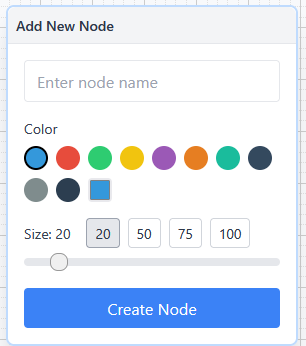
\includegraphics[width=0.5\linewidth]{Images/inputdialog.png}
    \caption{Dialog pro přidání nového vrcholu}
    \label{fig:input}
\end{figure}
\subsection{Selekce vrcholů a hran}
Existuje hned několik způsobů, jak vybrat prvky. Pro vybrání jedné hrany nebo vrcholu na ně stačí kliknout levým tlačítkem myši. Pokud jich chceme vybrat více, musíme u toho držet \textit{LShift}.
\par
Dále můžeme hrany vybrat pomocí obdélníkového výběru, který aktivujeme klávesou \textit{Ctrl} a tažením myši při držení stisknutého levého tlačítka, viz obrázek \ref{fig:select}.
\begin{figure}[h]
    \centering
    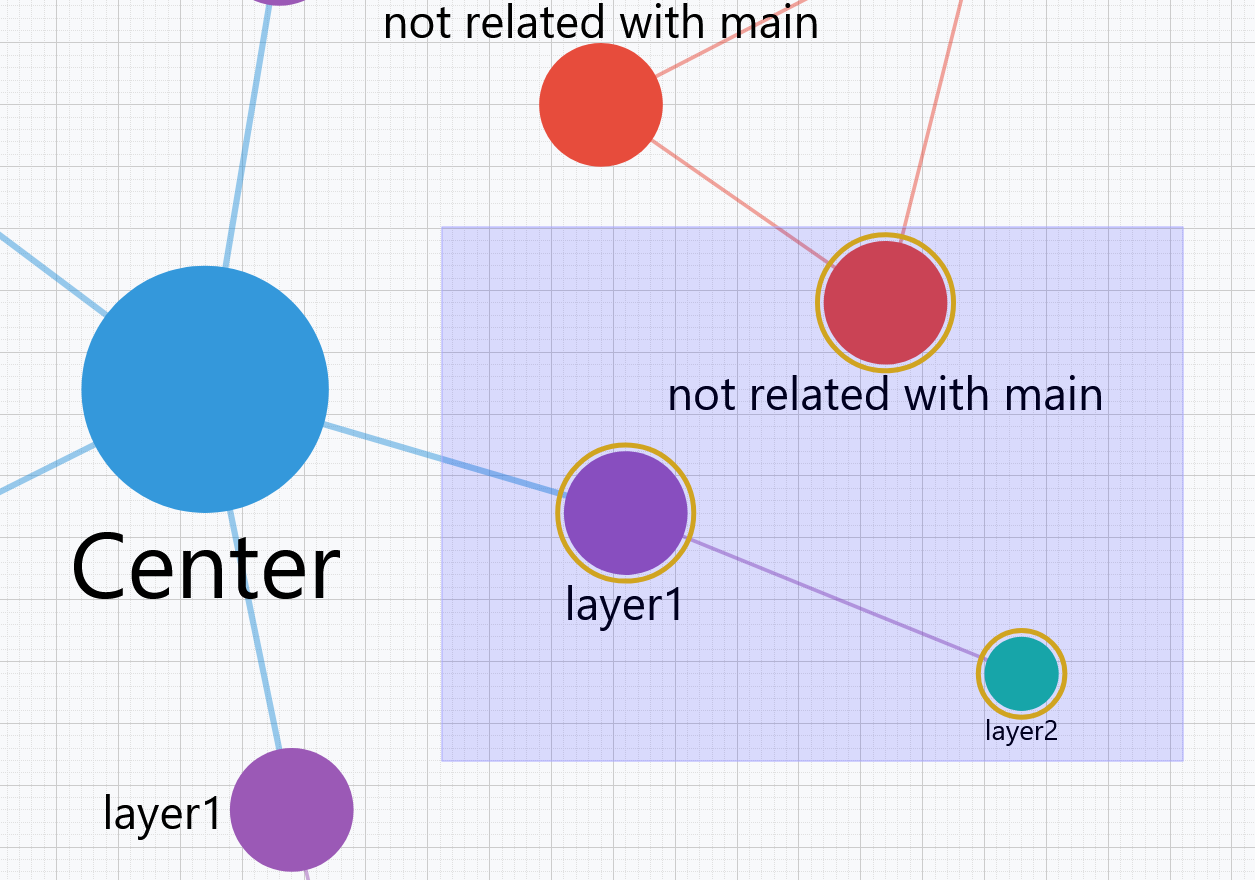
\includegraphics[width=0.5\linewidth]{Images/select.png}
    \caption{Obdélník pro selekci vrcholů}
    \label{fig:select}
\end{figure}
\par
Další speciální způsob, jak označit vrcholy, je pomocí \textit{wave selectu}, který postupně rekurzivně označí vrcholy spojené s těmi již označenými. Vždy je zde časová prodleva, než se vybere další vrstva, postupně je tato prodleva snižována; pro případy, kdy chce uživatel takto označit velké množství vrcholů. Selekce probíhá, pokud uživatel drží klávesu \textit{W}, pokud ji pustí, dojde k přerušení a další vrcholy nebudou vybrány. Tato funkcionalita se zejména hodí, pokud naše myšlenková mapa má strukturu lesa, má tedy hodně oddělených stromů - jednoduše se tak dá vybrat právě jeden celý strom.
\par
Poslední způsob, jak vybrat vrcholy, je pomocí vyhledávání. Automaticky se budou vybírat ty vrcholy, které obsahují zadaný řetězec.
\par
Pro odznačení jakéhokoliv výběru stačí kliknout levým tlačítkem myši na pozadí.
\newpage
\subsection{Přidání hran mezi vrcholy}
Pokud máme označené dva vrcholy, pomocí mezerníku je spojíme. Pokud máme označeny 3 nebo více vrcholů, po zmáčknutí mezerníku se spojí všechny vybrané vrcholy s tím, co bylo označeno jako první. Pokud chceme spojit všechny vrcholy mezi sebou, stačí zmáčknout najednou \textit{Ctrl} a mezerník.

\subsection{Odebrání vrcholu a hran}
Po stisknutí klávesy \textit{backspace} dojde k smazání vybraných prvků, nezáleží na tom, jestli jde o hrany nebo vrcholy. Pokud ovšem chceme smazat hrany, které mezi sebou sdílí vybrané vrcholy, dosáhneme toho tím stisknutím \textit{ctrl} a \textit{backspace}.
\subsection{Úprava vrcholu}
Pro úpravu vrcholu na něj dvojklikněme levým tlačítkem myši nebo pomocí klávesové kombinace \textit{ctrl} a \textit{Enter}. Objeví se nám dialog pro úpravu vrcholu (obrázek \ref{fig:edit}), který je předvyplněný jeho aktuálními parametry. Tento dialog se dá posouvat za jeho záhlaví a pro jeho zmizení stačí kliknout mimo něj.
\begin{figure}[h]
    \centering
    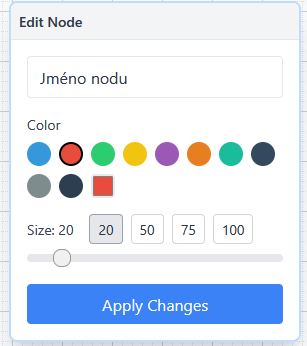
\includegraphics[width=0.5\linewidth]{Images/style.png}
    \caption{Dialog pro úpravu vrcholu}
    \label{fig:edit}
\end{figure}
\subsection{Undo a Redo}
Pro odčinění poslední akce stiskněte klávesovou kombinaci \textit{Ctrl} a \textit{Z}. Pokud jsme se vrátili o pár akcí do minulosti v historii provedených kroků, můžeme se pohybovat zpět k současnému bodu pomoci kombinace kláves \textit{Ctrl}, \textit{LShift} a \textit{Z}
\subsection{Změna layoutu}
Pomocí tlačítka Force Layout a Grid Layout (záleží, co je aktuálně vybráno) můžeme tyto dva režimy přepínat.
\subsection{Uložení}
Pro uložení neslouží žádná klávesová zkratka, ale tlačítko Save. Nebo stačí, pokud nebudeme dělat žádné změny po dobu delší než 2 vteřiny. 
\subsection{Seznam všech klávesových zkratek}
\label{seznam}
Veškeré klávesové zkratky naleznete na obrázku \ref{fig:shortcuts}; samotná webová stránka nabízí možnost zobrazení této nápovědy.
\begin{figure}[h]
    \centering
    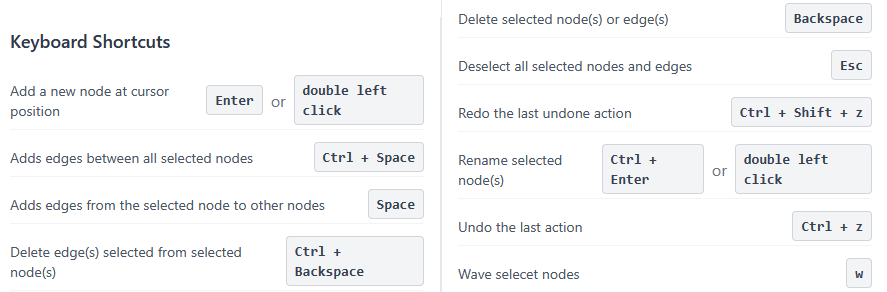
\includegraphics[width=1.1\linewidth]{Images/shortcuts.png}
    \caption{Seznam klávesových zkratek}
    \label{fig:shortcuts}
\end{figure}
